% Deployment chapter continued
\section{Bastion Host}
* according to the wikipedia arcticle, a person named Marcus J. Ranum defined the term 'bastion host' while discussing a article on firewalls as 
    * "...a system identified by the firewall administrator as a critical strong point in the network security. Generally, bastion hosts will have some degree of extra attention paid to their security, may undergo regular audits, and may have modified software."
* In context of AWS, a baston host sole purpose is to provide access to private network from external network such as internet. In a typical AWS VPC setup, an instance in a public subnet with a security group that includes a inbound rule to accept SSH traffic from trusted client host establishes secure remote connectivity after which the instance(bastion host) acts a jumping point to ssh into various private instances belonging to various private subnets within its VPC. 
* With bastion host in place, a administrator can(should) use ssh-agent forwarding to authenticate to private instances. Agent forwarding doesn't require administrator to store private keys on the bastion host and AWS best practices forbids storing private key files on servers.
* Another benefit bastion hosts provide is not having to expose various management ports to internet to configure utility/application services on private instances of the infrastructure.

Discuss ssh port-forwarding and showcase ssh config(a.k.a code/image of config)

\pagebreak

\section{SSH Tunnels}
Include source in references and cite it.
\begin{figure}[h!]
  \centering
  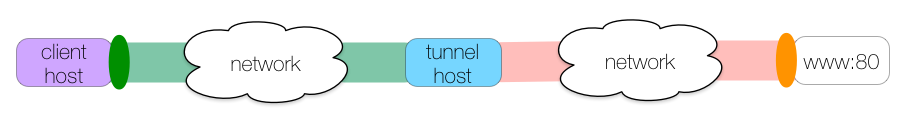
\includegraphics[width=15cm,height=5cm,keepaspectratio]{../media/crawler/simple-tunnel.png}
  \caption{simple tunnel}
  \label{fig:simpletunnel}
\end{figure}

figures
\begin{figure}[h!]
  \centering
  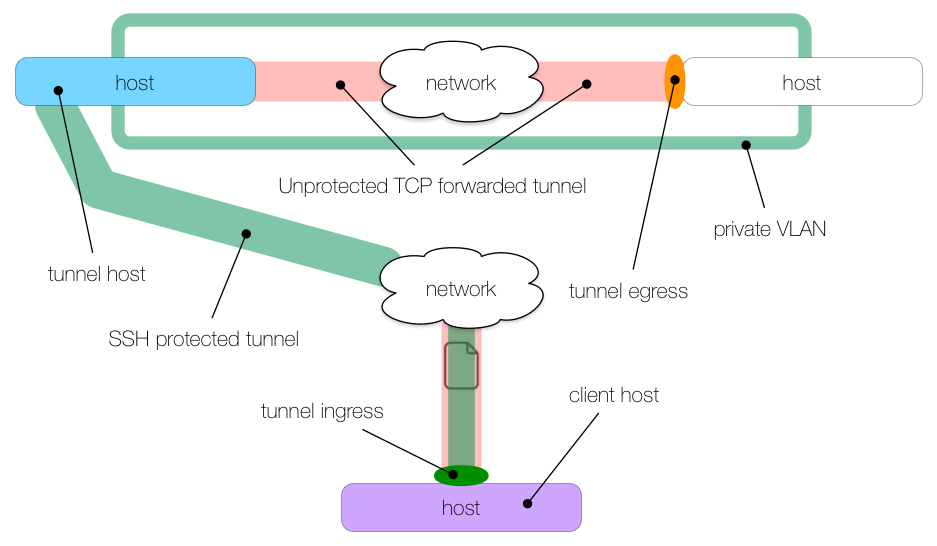
\includegraphics[width=15cm,height=12cm,keepaspectratio]{../media/crawler/ssh-tunnel-host-access.png}
  \caption{poor man's VPN}
  \label{fig:poormanvpn}
\end{figure}